\documentclass[a4paper, 12pt]{article}
\usepackage[a4paper,top=1.5cm, bottom=1.5cm, left=1cm, right=1cm]{geometry}

% Работа с русским языком
\usepackage[utf8]{inputenc}
\usepackage{mathtext}                % русские буквы в формулах
\usepackage[english, russian]{babel} % локализация и переносы

\usepackage{graphicx}   % Вставка изображений
\usepackage{float}      % "Плавающие" изображения
\usepackage{wrapfig}    % Обтекание фигур (таблиц, картинок и прочего)
\graphicspath{ {./images/} }

\usepackage{multirow}
\usepackage{amsmath}
\usepackage{amsfonts}
\usepackage{indentfirst}
\usepackage{longtable}
\graphicspath{{pictures/}}
\usepackage{natbib}

%%% Колонтитулы
\usepackage{titleps}
\newpagestyle{main}{
	\setheadrule{0.4pt}
	\sethead{Отчёт о выполнении лабораторной работы 2.1.3}{}{}
	\setfootrule{0.4pt}                       
	\setfoot{ФРКТ МФТИ, 2023}{}{\thepage} 
}
\pagestyle{main}  

\title{Работа 2.1.3 \\ Определение $C_p/C_v$ по скорости звука в газе}
\author{Дмитрий Тихонов, ФРКТ, Б01-206}
\date{1 марта 2023 г.}

\begin{document}
    \begin{titlepage}
	\begin{center}
            {\large МОСКОВСКИЙ ФИЗИКО-ТЕХНИЧЕСКИЙ ИНСТИТУТ (НАЦИОНАЛЬНЫЙ       ИССЛЕДОВАТЕЛЬСКИЙ УНИВЕРСИТЕТ)}
	\end{center}
 
	\begin{center}
		{\large Физтех-школа радиотехники и компьютерных технологий}
	\end{center}
	
	\vspace{8cm}
	{\LARGE
		\begin{center}
                {\bf Отчёт о выполнении лабораторной работы 2.1.3}\\
                Определение $C_p/C_v$ по скорости звука в газе
		\end{center}
	}
	\vspace{5cm}
	\begin{flushright}
		{\Large Автор:\\ Тихонов Дмитрий Романович, \\
			\vspace{0.2cm}
			студент группы Б01-206}
	\end{flushright}
	\vspace{5cm}
	\begin{center}
		\Large Долгопрудный, 2023
	\end{center}
    \end{titlepage}

    \section*{Введение}
        \noindent \textbf{Цель работы:}  
            \begin{enumerate}
                \item измерение частоты колебаний и длины волны при резонансе звуковых колебаний в газе, заполняющем трубу;
                \item определение показателя адиабаты с помощью уравнения состояния идеального газа.
            \end{enumerate}

        \noindent \textbf{В работе используются:} звуковой генератор ГЗ; электронный осциллограф ЭО; микрофон; телефон; раздвижная труба; баллон со сжатым углекислым газом; газгольдер.

    \section*{Теоретические сведения}

        \noindent Скорость распространения звуковой волны в газах зависит от показателя адиабаты $\gamma$. На измерении скорости звука основан один из наиболее точных методов определения показателя адиабаты. Скорость звука в газах определяется формулой:

        \begin{equation}\label{velocity}
            c=\sqrt{\gamma\frac{RT}{\mu}}.
        \end{equation}
        \noindent где $R$ -- газовая постоянная, $T$ -- температура газа, а $\mu$ -- его молярная масса. Преобразуя эту формулу, найдем
        
        \begin{equation}
            \label{gamma}
            \boxed{\gamma = \frac{\mu}{RT}c^2}.
        \end{equation}

        \noindent Таким образом, для определения показателя адиабаты достаточно измерить температуру газа и скорость распространения звука (молярная масса газа предполагается известной).\\

        \noindent Звуковая волна, распространяющаяся вдоль трубы, испытывает многократные отражения от торцов. Звуковые колебания в трубе являются наложением всех отраженных волн и очень сложны. Картина упрощается, если длина трубы $L$ равна целому числу полуволн, то есть когда \[ L=n\lambda/2, \] где $\lambda$ -- длина волны звука в трубе, а $n$ -- любое целое число. Если это условие выполнено, то волна, отраженная от торца трубы, вернувшаяся к ее началу и вновь отраженная, совпадает по фазе с падающей. Совпадающие по фазе волны усиливают друг друга. Амплитуда звуковых колебаний при этом резко возрастает -- наступает резонанс.\\

        \noindent При звуковых колебаниях слои газа, прилегающие к торцам трубы, не испытывают смещения (\textit{узлы смещения}). Узлы смещения повторяются по всей длине трубы через $\lambda/2$. Между узлами находятся максимумы смещения (\textit{пучности}).\\

        \noindent Скорость звука c связана с его частотой $f$ и длиной волны $\lambda$ соотношением

        \begin{equation}
            \label{lambda_f}
            c=\lambda f.
        \end{equation}

    \section*{Методика измерений и используемое оборудование}

         \noindent При неизменной частоте $f$ звукового генератора (а следовательно, и неизменной длине звуковой волны $\lambda$) можно изменять длину трубы $L$. Для этого применяется раздвижная труба. Длина раздвижной трубы постепенно увеличивается, и наблюдается ряд последовательных резонансов. Возникновение резонанса легко наблюдать на осциллографе по резкому увеличению амплитуды колебаний. Для последовательных резонансов имеем 
                
        \begin{equation}
            \label{first}
            L_n=n\frac{\lambda}{2}, \quad L_{n+1}=(n+1)\frac{\lambda}{2}, \quad \dots, \quad L_{n+k} = n\frac{\lambda}{2}+k\frac{\lambda}{2},
        \end{equation} 
        \noindent т. е. $\lambda/2$ равно угловому коэффициенту графика, изображающего зависимость длины трубы $L$ от номера резонанса $k$. Скорость звука находится по формуле \eqref{lambda_f}.\\
    
        \noindent Схема установки ппредставлена на рис. \ref{setup}. Установка содержит раздвижную трубу с миллиметровой шкалой. Через патрубок (на рисунке не показан) труба может наполняться воздухом или углекислым газом из газгольдера. На этой установке производятся измерения $\gamma$ для воздуха и для $CO_2$. Звуковые колебания в трубе возбуждаются телефоном Т и улавливаются микрофоном М. Мембрана телефона приводится в движение переменным током звуковой частоты; в качестве источника переменной ЭДС используется звуковой генератор ГЗ. Возникающий в микрофоне сигнал наблюдается на осциллографе ЭО.\\
    
       \noindent  Микрофон и телефон присоединены к установке через тонкие резиновые трубки. Такая связь достаточна для возбуждения и обнаружения звуковых колебаний в трубе и в то же время мало возмущает эти колебания: при расчетах оба торца трубы можно считать неподвижными, а влиянием соединительных отверстий пренебречь.
    
        \begin{figure}[H]
            \centering
            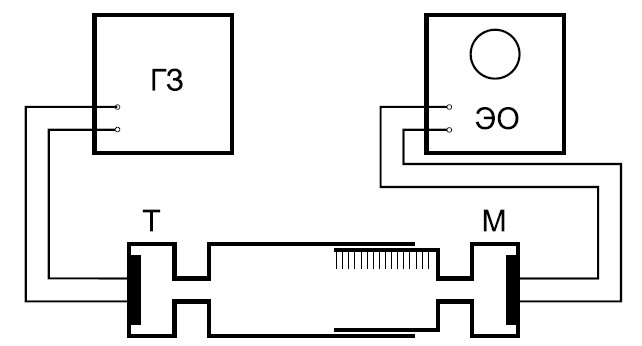
\includegraphics[width=12cm]{images/setup.jpg}
            \caption{Установка для измерения скорости звука при помощи раздвижной трубы}
            \label{setup}
        \end{figure}
    
    \section*{Результаты измерений и обработка данных}
    
        \subsection*{Измерение $C_p/C_v$ для воздуха при помощи установки с раздвижной трубой}

            \noindent Проведём измерение коэффициента $C_p/C_v$ для воздуха при помощи установки с раздвижной трубой. Для проведения серии измерений фиксируем частоту звукового сигнала и оставляем её неизменной до окончания снятия показаний. Увеличиваем и уменьшаем длину трубки, чтобы добиться резонанса, возникновение которого устанавливается при помощи осциллографа. При возникновении резонанса фиксируем то расстояние, на которое была выдвинута трубка прибора. Данные измерения проводим для нескольких значений частот. Полученные результаты заносим в таблицу \ref{tab:oxy1} и в таблицу \ref{tab:oxy2}.

            \begin{table}[H]
                \centering
                
                \begin{tabular}{|c|cc|cc|cc|cc|cc|}
                    \hline
                    f, Гц & \multicolumn{2}{c|}{2705}& \multicolumn{2}{c|}{3024}& \multicolumn{2}{c|}{3304}& \multicolumn{2}{c|}{3640} & \multicolumn{2}{c|}{4019} \\ \hline
                    
                   $k$ & \multicolumn{1}{c|}{$l_k$, мм} & $\Delta L$, мм & \multicolumn{1}{c|}{$l_k$, мм} & $\Delta L$, мм & \multicolumn{1}{c|}{$l_k$, мм} & $\Delta L$, мм & \multicolumn{1}{c|}{$l_k$, мм} & $\Delta L$, мм & \multicolumn{1}{c|}{$l_k$, мм} & $\Delta L$, мм \\ \hline
                   
                    0 & \multicolumn{1}{c|}{38} & 0 & \multicolumn{1}{c|}{11}       & 0 & \multicolumn{1}{c|}{9} & 0 & \multicolumn{1}{c|}{34} & 0 & \multicolumn{1}{c|}{10} & 0 \\ \hline
                    
                    1 & \multicolumn{1}{c|}{104} & 66 & \multicolumn{1}{c|}{66} & 55 & \multicolumn{1}{c|}{57} & 48 & \multicolumn{1}{c|}{81} & 47 & \multicolumn{1}{c|}{53} & 43 \\ \hline
                    
                    2 & \multicolumn{1}{c|}{163} & 125 & \multicolumn{1}{c|}{123} & 112 & \multicolumn{1}{c|}{109} & 100 & \multicolumn{1}{c|}{127} & 93 & \multicolumn{1}{c|}{95} & 85 \\ \hline
                    
                    3 & \multicolumn{1}{c|}{227} & 189 & \multicolumn{1}{c|}{179} & 168 & \multicolumn{1}{c|}{161} & 152 & \multicolumn{1}{c|}{175} & 141 & \multicolumn{1}{c|}{133} & 123 \\ \hline
                    
                    4 & \multicolumn{1}{c|}{} & & \multicolumn{1}{c|}{} & & \multicolumn{1}{c|}{212} & 203 & \multicolumn{1}{c|}{223} & 189 & \multicolumn{1}{c|}{180} & 170 \\ \hline
                    
                    5 & \multicolumn{1}{c|}{} & & \multicolumn{1}{c|}{} & & \multicolumn{1}{c|}{} & & \multicolumn{1}{c|}{} &          & \multicolumn{1}{c|}{} & \\ \hline
                \end{tabular}
                \caption{Результаты измерений для воздуха}
                \label{tab:oxy1}
            \end{table}

            \begin{table}[H]
                \centering
                
                \begin{tabular}{|c|cc|cc|}
                    \hline
                    $f$, Гц & \multicolumn{2}{c|}{4408} & \multicolumn{2}{c|}{4803} \\ \hline
                    
                    $k$ & \multicolumn{1}{c|}{$l_k$, мм} & $\Delta L$, мм & \multicolumn{1}{c|}{$l_k$, мм} & $\Delta L$, мм \\ \hline
                    
                    0 & \multicolumn{1}{c|}{22} & 0 & \multicolumn{1}{c|}{20}       & 0        \\ \hline
                    
                    1 & \multicolumn{1}{c|}{60} & 38 & \multicolumn{1}{c|}{56}       & 36 \\ \hline
                    
                    2 & \multicolumn{1}{c|}{101} & 79 & \multicolumn{1}{c|}{92} & 72 \\ \hline
                    
                    3 & \multicolumn{1}{c|}{140} & 118 & \multicolumn{1}{c|}{128} & 108 \\ \hline
                    
                    4 & \multicolumn{1}{c|}{179} & 157 & \multicolumn{1}{c|}{164} & 144 \\ \hline
                    
                    5 & \multicolumn{1}{c|}{229} & 207 & \multicolumn{1}{c|}{200} & 180 \\ \hline
                \end{tabular}
                \caption{Результаты измерений для воздуха (\textit{продолжение})}
                \label{tab:oxy2}
            \end{table}

            \noindent Для каждого измерения погрешность измерения \textit{выдвига} трубы равна $\sigma_l = 0,5$ мм. Также для каждого измерения вычислим $\Delta L = l_k - l_0$. Погрешность определения этой величины составит $\sigma_L=~\sqrt{2}\sigma_l \approx 0,7$ мм. По полученным данным построим графики зависимости $L_k(k)$ (рис. \ref{graph1}). Так как погрешность измерения $\Delta L$ мала по сравнению с масштабом графика, кресты погрешности не были нанесены на график.

            \begin{figure}[H]
                \centering
                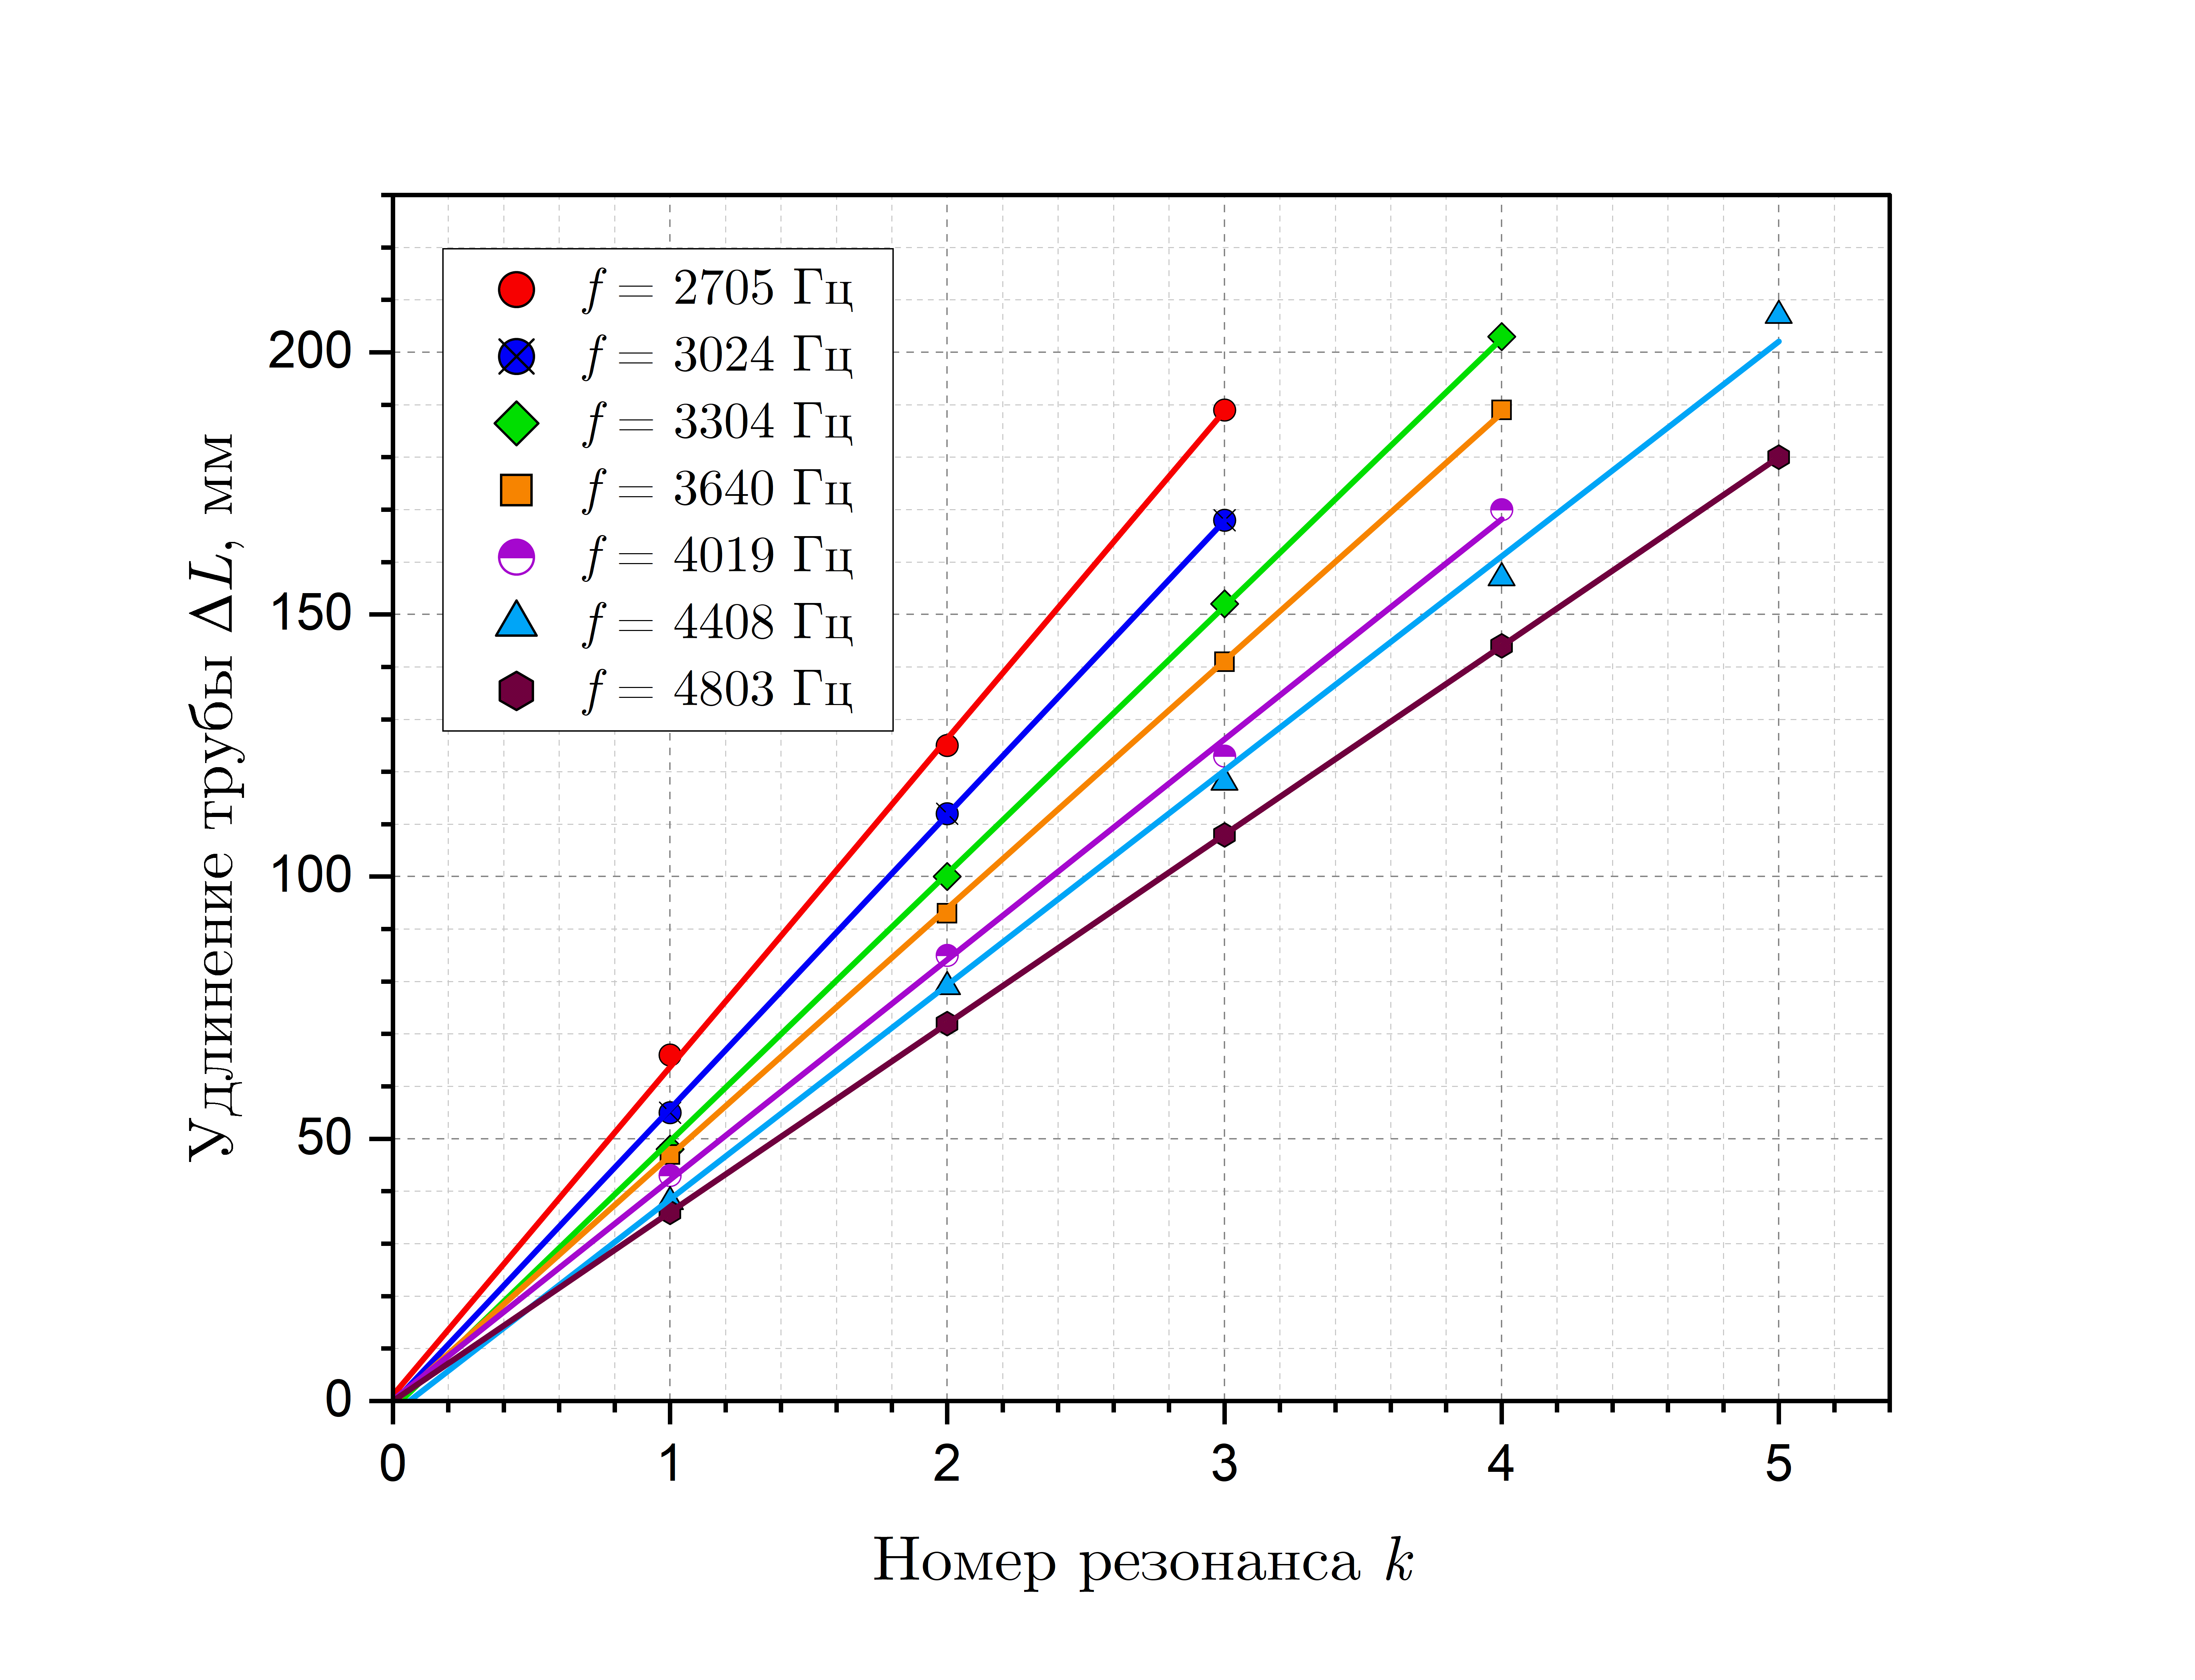
\includegraphics[scale = 0.5]{images/L(k).png}
                \caption{График зависимости $L(k)$ для воздуха}
                \label{graph1}
            \end{figure}

            \noindent Аппроксимируем полученные зависимости прямыми $y=ax$ используя метод наименьших квадратов. Коэффициент $a$ находим согласно следующей формуле:

             \begin{equation}                
                a=\frac{\left\langle kL_k \right\rangle}{\left\langle k^2 \right\rangle}.
            \end{equation}

            \noindent Случайную погрешность определения $ a $ оценим следующим образом:
            
            \begin{equation}
                \sigma^\text{случ}_a=\sqrt{\frac{1}{N-1}\left(\frac{\left\langle L_k^2 \right\rangle}{\left\langle k^2 \right\rangle}-a^2\right)},
            \end{equation}
            \noindent где $N$ -- количество измерений. Систематическая погрешность определения $a$ равна $\sigma_a^\text{сист} = \sigma_{L_k}$. Тогда полная погрешность определения коэффициента $a$ может быть вычислена по следующей формуле:

            \begin{equation}
                \sigma^\text{случ}_a=\sqrt{\frac{1}{N-1}\left(\frac{\left\langle L_k^2 \right\rangle}{\left\langle k^2 \right\rangle}-a^2\right)},
            \end{equation}

            \noindent Используя эти формулы вычисляем коэффициенты $a$ для каждого значения частоты $f$. Результаты вычислений заносим в таблицу \ref{tab:resSpeed}.

            \begin{table}[H]
                \centering
                \begin{tabular}{|c|c|c|c|c|c|c|}
                    \hline
                    $f$, Гц & $a$, мм & $\sigma_a$, мм & $\lambda$, мм & $\sigma_\lambda$, мм & $c$, м/с & $\sigma_c$, м/с \\ \hline
                    2705 & 62,6 & 0,9 & 125,2 & 1,8 & 338,7 & 4,9 \\ \hline
                    3024 & 56,1 & 0,3 & 112,2 & 0,5 & 339,3 & 1,6 \\ \hline
                    3304 & 51,0 & 0,4 & 102,0 & 0,8 & 337,0 & 2,8 \\ \hline
                    3640 & 47,2 & 0,2 & 94,4  & 0,5 & 343,6 & 1,7 \\ \hline
                    4019 & 42,0 & 0,7 & 84,0  & 1,4 & 337,6 & 5,6 \\ \hline
                    4408 & 40,0 & 1,0 & 80,0  & 1,8 & 352,6 & 7,9 \\ \hline
                    4803 & 36,0 & 0,0 & 72,0  & 0,0 & 345,8 & 0,0 \\ \hline
                \end{tabular}
                \caption{Результаты вычислений скорости звука для воздуха}
                \label{tab:resSpeed}
            \end{table}

            \noindent Согласно \eqref{first}, угловой коэффициент наклона прямой $a$ равен $\lambda/2$.

            \noindent Скорость звука в воздухе можно вычислить по следующей формуле: 
            \[ c = \lambda f. \]
            
            \noindent Погрешность такого вычисления равна (при этом в каждом измерении примем $\sigma_f \approx 1$ Гц)
            \[ \sigma_c=c\sqrt{\varepsilon_f^2+\varepsilon_\lambda^2}. \]
            
            \noindent Эти результаты также заносим в таблицу \ref{tab:resSpeed}.
            
            \noindent Таким образом, мы получили значение $c$ для каждого отдельного значения частоты. Усредняя вычисленные значения, в итоге получаем \[\boxed{ c = (342,1 \pm 3,5) \text{ м/с}}\quad (\varepsilon=1\%) \]
            
            \noindent Также, по формуле \eqref{gamma}, вычислим $ C_p/C_v $:
            \[ \frac{C_p}{C_v} = \gamma = \frac{\mu}{RT}c^2. \]
            
            \noindent При этом для воздуха $ \displaystyle \mu \approx 0,02898 \text{ } \frac{\text{кг}}{\text{моль}} $. Во время эксперимента температура в лаборатории равнялась $T = 25 \text{ } ^\circ C$. Тогда погрешность такого вычисления можно оценить по следующей формуле:
            \[ \sigma_\gamma = \sqrt{2}\varepsilon_c\gamma.\]
            
            \noindent В итоге получаем:
            \[ \boxed{\gamma = 1,37 \pm 0,03}\quad (\varepsilon=1,5\%) \]

        \subsection*{Измерение $C_p/C_v$ для углекислого газа при помощи установки с раздвижной трубой}
            
            \noindent В этой части работы проведём измерения, аналогичные проведённым с воздухом, но теперь для трубы, заполненной углекислым газом. Измерения резонансных максимумов с углекислым газом будем производить при малых перемещениях подвижной части трубы как внутрь, так и наружу. Заносим результаты измерений зависимости номера резонанса от величины, на которую выдвинута труба, в таблицу \ref{tab:CO2_1} и таблицу \ref{tab:CO2_2}.

            \begin{table}[H]
                \centering
                \begin{tabular}{|c|cc|cc|cc|cc|cc|}
                    \hline
                    
                    $f$, Гц & \multicolumn{2}{c|}{2016} & \multicolumn{2}{c|}{2189} & \multicolumn{2}{c|}{2391} & \multicolumn{2}{c|}{2628} & \multicolumn{2}{c|}{2830} \\ \hline
                    
                    $k$ & \multicolumn{1}{c|}{$l_k$, мм} & $\Delta L$, мм & \multicolumn{1}{c|}{$l_k$, мм} & $\Delta L$, мм & \multicolumn{1}{c|}{$l_k$, мм} & $\Delta L$, мм & \multicolumn{1}{c|}{$l_k$, мм} & L\_k, мм & \multicolumn{1}{c|}{$l_k$, мм} & $\Delta L$, мм \\ \hline
                    
                    0 & \multicolumn{1}{c|}{0} & 0 & \multicolumn{1}{c|}{15}       & 0 & \multicolumn{1}{c|}{32} & 0 & \multicolumn{1}{c|}{51} & 0 & \multicolumn{1}{c|}{41} & 0 \\ \hline
                    
                    0 & \multicolumn{1}{c|}{0} & 0 & \multicolumn{1}{c|}{39}       & 24 & \multicolumn{1}{c|}{42} & 10 & \multicolumn{1}{c|}{54} & 3 & \multicolumn{1}{c|}{52} & 11 \\ \hline
                    
                    1 & \multicolumn{1}{c|}{64} & 64 & \multicolumn{1}{c|}{86} & 71 & \multicolumn{1}{c|}{102} & 70 & \multicolumn{1}{c|}{115} & 64 & \multicolumn{1}{c|}{103} & 62 \\ \hline
                    
                    1 & \multicolumn{1}{c|}{76} & 76 & \multicolumn{1}{c|}{99} & 84 & \multicolumn{1}{c|}{109} & 77 & \multicolumn{1}{c|}{118} & 67 & \multicolumn{1}{c|}{108} & 67 \\ \hline
                    
                    2 & \multicolumn{1}{c|}{146} & 146 & \multicolumn{1}{c|}{162} & 147 & \multicolumn{1}{c|}{173} & 141 & \multicolumn{1}{c|}{179} & 128 & \multicolumn{1}{c|}{162} & 121 \\ \hline
                    
                    2     & \multicolumn{1}{c|}{153} & 153 & \multicolumn{1}{c|}{170} & 155 & \multicolumn{1}{c|}{175} & 143 & \multicolumn{1}{c|}{181} & 130 & \multicolumn{1}{c|}{167} & 126 \\ \hline
                    
                    3 & \multicolumn{1}{c|}{225} & 225 & \multicolumn{1}{c|}{} & & \multicolumn{1}{c|}{} & & \multicolumn{1}{c|}{} & & \multicolumn{1}{c|}{222} & 181 \\ \hline
                    
                    3 & \multicolumn{1}{c|}{225} & 225 & \multicolumn{1}{c|}{} & & \multicolumn{1}{c|}{} & & \multicolumn{1}{c|}{} & & \multicolumn{1}{c|}{223} & 182      \\ \hline
                    
                    4 & \multicolumn{1}{c|}{} & & \multicolumn{1}{c|}{} & & \multicolumn{1}{c|}{} & & \multicolumn{1}{c|}{} & & \multicolumn{1}{c|}{} & \\ \hline
                    
                    4 & \multicolumn{1}{c|}{} & & \multicolumn{1}{c|}{} & & \multicolumn{1}{c|}{} & & \multicolumn{1}{c|}{} & & \multicolumn{1}{c|}{} & \\ \hline
                    
                \end{tabular}
                \caption{Результаты измерений для углекислого газа}
                \label{tab:CO2_1}
            \end{table}
                
            \begin{table}[H]
                \centering
                \begin{tabular}{|c|cc|cc|}
                    \hline
                    $f$, Гц & \multicolumn{2}{c|}{3032} & \multicolumn{2}{c|}{3263} \\ \hline
                    $k$ & \multicolumn{1}{c|}{$l_k$, мм} & $\Delta L$, мм & \multicolumn{1}{c|}{$l_k$, мм} & $\Delta L$, мм \\ \hline
                    0     & \multicolumn{1}{c|}{5} & 0 & \multicolumn{1}{c|}{15}       & 0 \\ \hline
                    0 & \multicolumn{1}{c|}{7} & 2 & \multicolumn{1}{c|}{17}       & 2 \\ \hline
                    1     & \multicolumn{1}{c|}{59} & 54 & \multicolumn{1}{c|}{65} & 50 \\ \hline
                    1 & \multicolumn{1}{c|}{61} & 56 & \multicolumn{1}{c|}{73} & 58 \\ \hline
                    2 & \multicolumn{1}{c|}{115} & 110 & \multicolumn{1}{c|}{118}      & 103 \\ \hline
                    2 & \multicolumn{1}{c|}{117} & 112 & \multicolumn{1}{c|}{122}      & 107 \\ \hline
                    3 & \multicolumn{1}{c|}{171} & 166 & \multicolumn{1}{c|}{170}      & 155 \\ \hline
                    3 & \multicolumn{1}{c|}{172} & 167 & \multicolumn{1}{c|}{171}      & 156      \\ \hline
                    4 & \multicolumn{1}{c|}{228} & 223 & \multicolumn{1}{c|}{224}      & 209 \\ \hline
                    4 & \multicolumn{1}{c|}{228} & 223 & \multicolumn{1}{c|}{225}      & 210 \\ \hline
                \end{tabular}
                \caption{Результаты измерений для углекислого газа (\textit{продолжение)}}
                \label{tab:CO2_2}
            \end{table}

            \noindent Строим графики зависимости $L_k(k)$ (рис. \ref{graph2}). Аппроксимируем зависимости прямыми $y=ax$. Результаты заносим в таблицу \ref{tab:resCO2}. Вычисляем также $\lambda$ и $c$ для каждого значения частоты $f$.

            \begin{figure}[H]
                \centering
                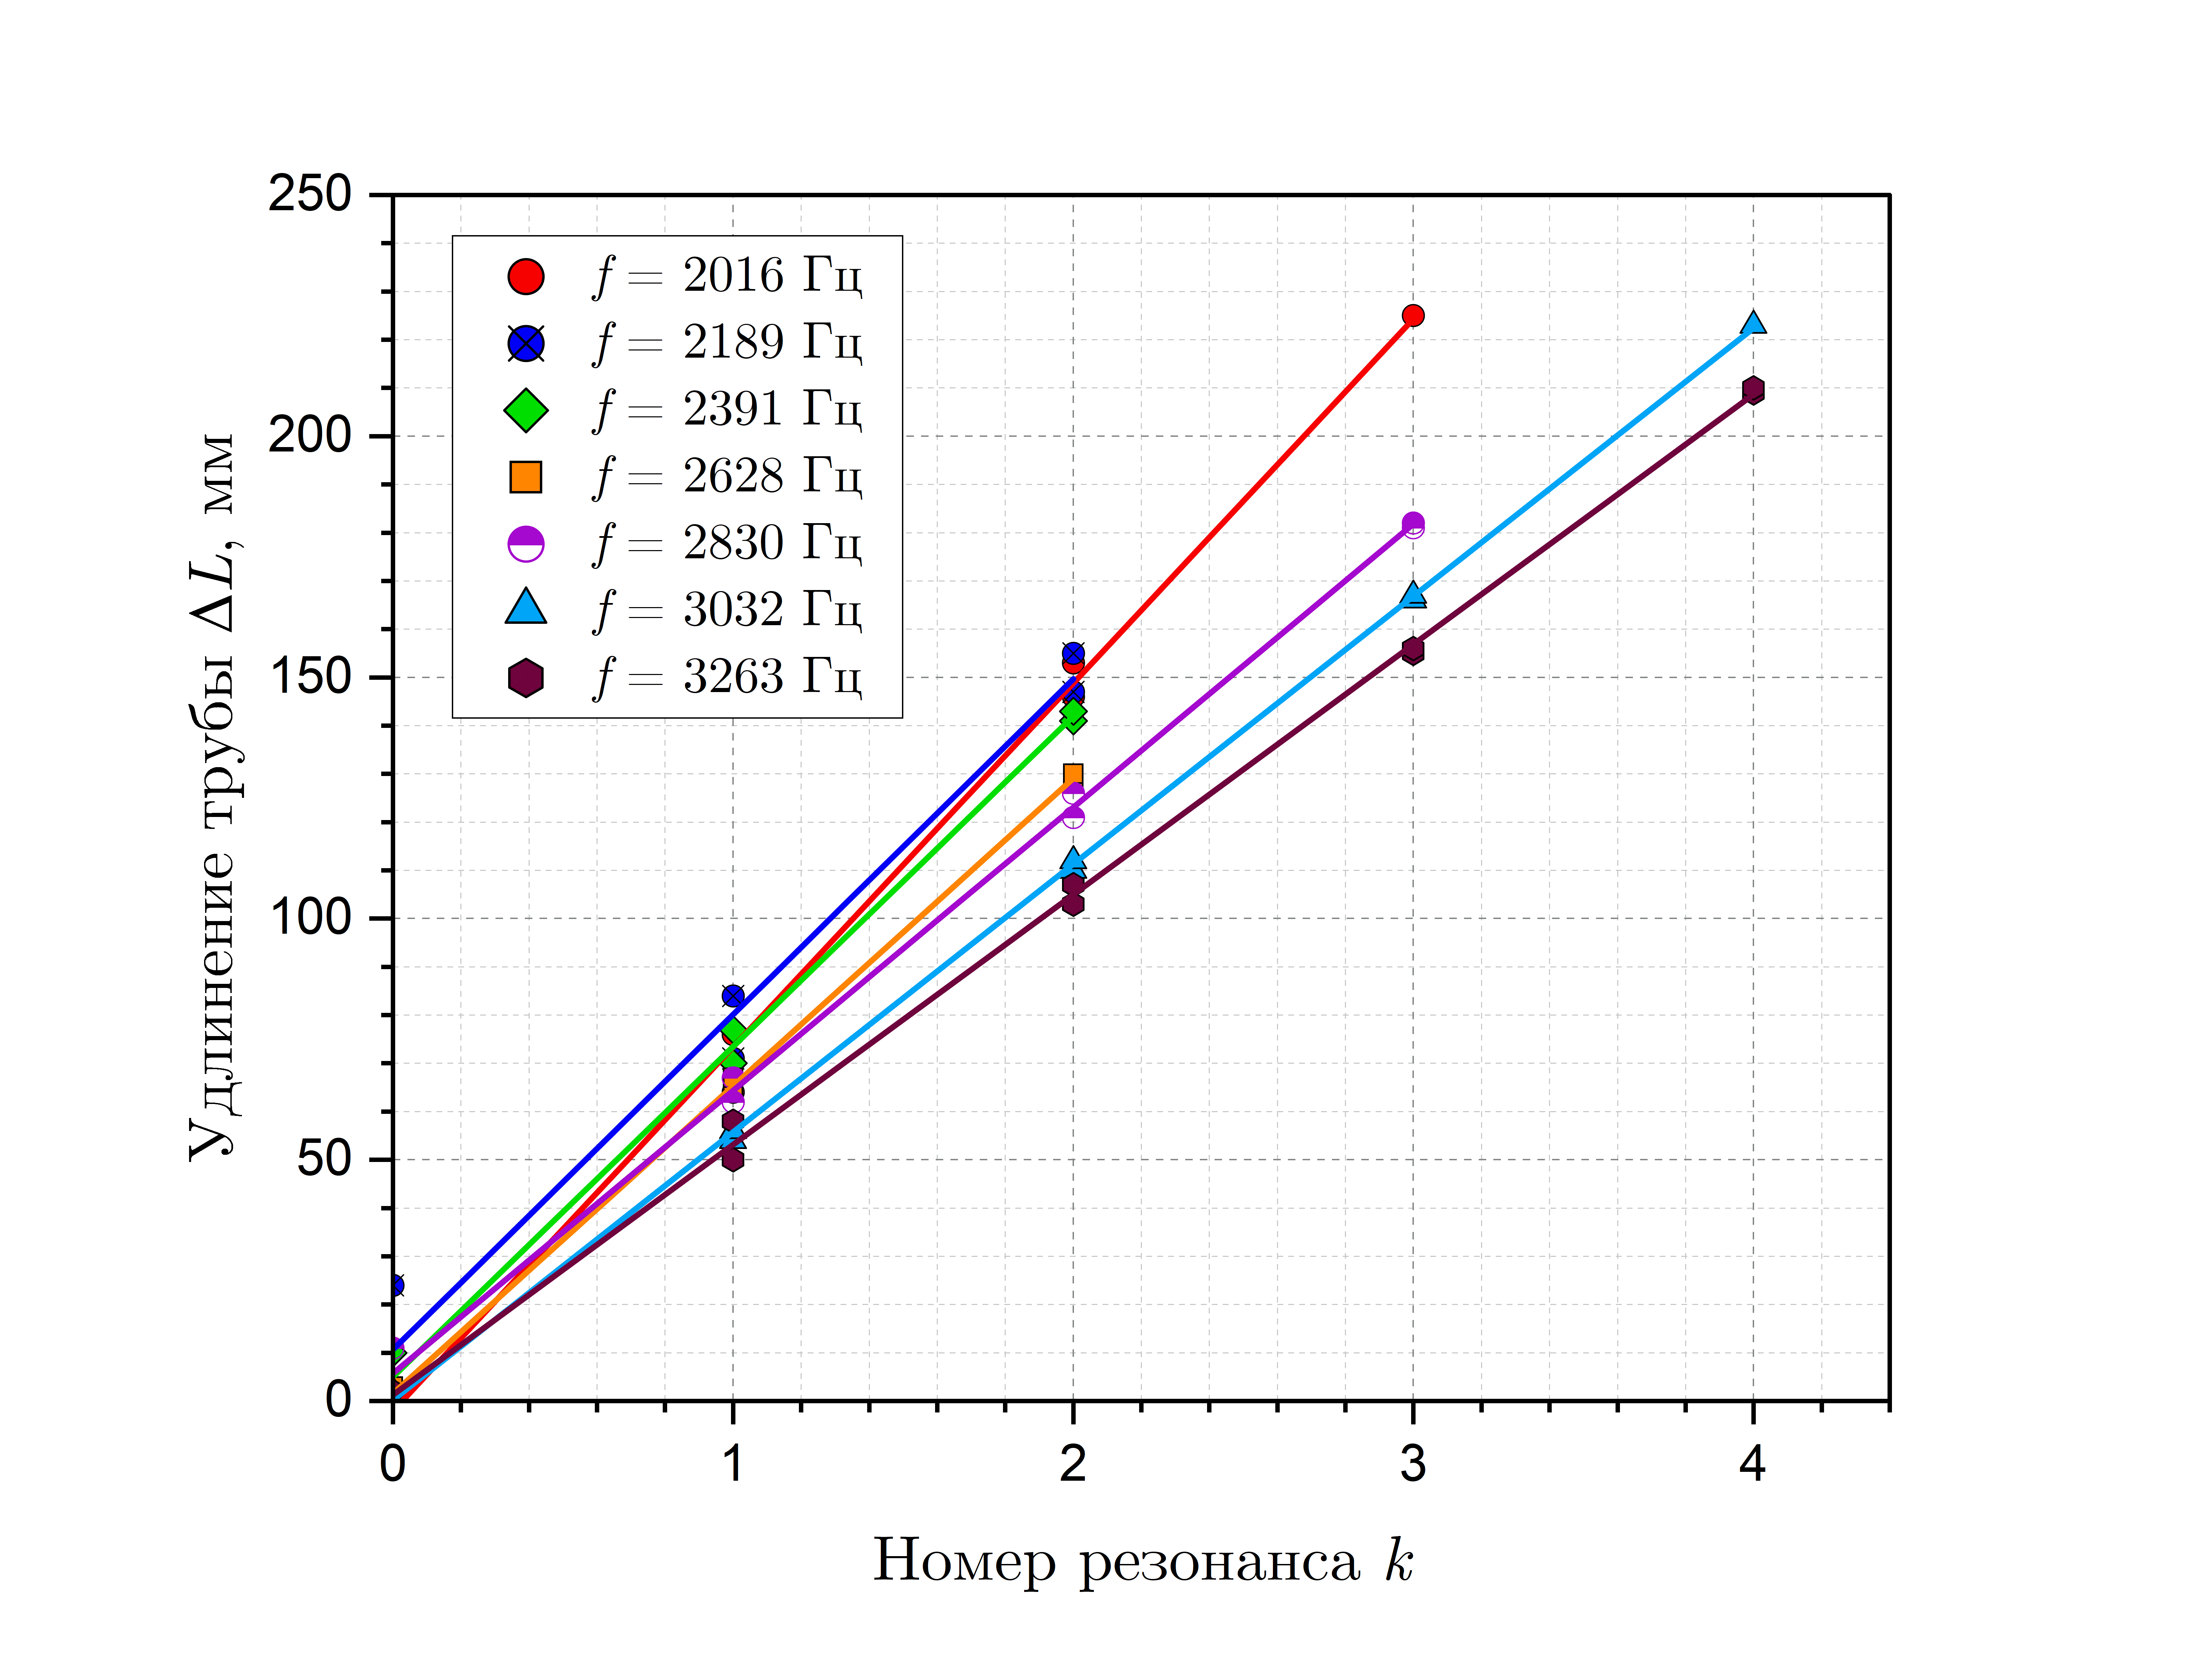
\includegraphics[scale = 0.5]{images/L(k)_CO2.png}
                \caption{График зависимости $L(k)$ для углекислого газа}
                \label{graph2}
            \end{figure}

            \begin{table}[H]
                \centering
                \begin{tabular}{|c|c|c|c|c|c|c|}
                \hline
                    $f$, Гц & $a$, мм & $\sigma_a$, мм & $\lambda$, мм & $\sigma_\lambda$, мм & $c$, м/с & $\sigma_c$, мм \\ \hline
                    2016 & 75,5 & 1,5 & 150,9 & 2,9  & 304,2 & 5,9   \\ \hline
                    2189 & 69,5 & 5,2 & 139,0 & 10,3 & 304,3 & 22,5  \\ \hline
                    2391 & 68,5 & 2,2 & 137,0 & 4,4  & 327,6 & 10,4  \\ \hline
                    2628 & 63,8 & 0,8 & 127,5 & 1,7  & 335,1 & 4,4   \\ \hline
                    2830 & 58,7 & 1,2 & 117,4 & 2,4 & 332,2 & 6,8    \\ \hline
                    3032 & 55,6 & 0,3 & 111,1 & 0,5 & 336,9 & 1,5    \\ \hline
                    3263 & 51,9 & 0,6 & 103,7 & 1,1 & 338,4 & 3,6    \\ \hline
                \end{tabular}
                \caption{Результаты вычислений для углекислого газа}
	        \label{tab:resCO2}
            \end{table}

            \noindent Усредняя результаты всех экспериментов, получаем:
            \[ \boxed{c=(325,5 \pm 7,7)  \text{ м/с}} \quad (\varepsilon=2,3\%)\]

            \noindent Вычисляя $C_p/C_v$ аналогично предыдущему пункту, получаем
            \[ \boxed{\gamma = 1,88 \pm 0,06}\quad (\varepsilon=3,3\%) \]

        \subsection*{Измерение $C_p/C_v$ для углекислого газа и воздуха при неизменной длине трубы и температуре}
        
            \noindent Проведём измерения $C_p/C_v$ для воздуха и углекислого газа при $T = const$. Для этого будем использовать трубу во \textit{вставленном состоянии}, размер которой $ L = (700 \pm 5) $ мм. Для фиксированной температуры будем изменять частоту звукового сигнала, тем самым изменяя и длину волны, так, чтобы мы могли наблюдать последовательные резонансы. Для каждого резонанса будем фиксировать частоту, при которой он возник. Измерения будем проводить при увеличении и уменьшении частоты. Полученные измерения занесём в таблицу \ref{tab:constL}.

            \begin{table}[H]
                \centering
                \begin{tabular}{|c|cc|cc|}
                    \hline
                    & \multicolumn{2}{c|}{Углекислый газ} & \multicolumn{2}{c|}{Воздух} \\ \hline
                    $k$ & \multicolumn{1}{c|}{$f_k$, Гц} & $f_{k}$', Гц & \multicolumn{1}{c|}{$f_k$, Гц} & $f_{k}$', Гц \\ \hline
                    0  & \multicolumn{1}{c|}{467}      & 468       & \multicolumn{1}{c|}{468}      & 469       \\ \hline
                    1  & \multicolumn{1}{c|}{731}      & 724       & \multicolumn{1}{c|}{727}      & 761       \\ \hline
                    2  & \multicolumn{1}{c|}{902}      & 902       & \multicolumn{1}{c|}{932}      & 947       \\ \hline
                    3  & \multicolumn{1}{c|}{1183}     & 1226      & \multicolumn{1}{c|}{1263}     & 1256      \\ \hline
                    4  & \multicolumn{1}{c|}{1384}     & 1371      & \multicolumn{1}{c|}{1445}     & 1441      \\ \hline
                    5  & \multicolumn{1}{c|}{1712}     & 1723      & \multicolumn{1}{c|}{1738}     & 1764      \\ \hline
                    6  & \multicolumn{1}{c|}{1816}     & 1831      & \multicolumn{1}{c|}{1804}     & 1973      \\ \hline
                    7  & \multicolumn{1}{c|}{2176}     & 2160      & \multicolumn{1}{c|}{2246}     & 2238      \\ \hline
                    8  & \multicolumn{1}{c|}{2385}     & 2345      & \multicolumn{1}{c|}{2478}     & 2492      \\ \hline
                    9  & \multicolumn{1}{c|}{2639}     & 2637      & \multicolumn{1}{c|}{2722}     & 2730      \\ \hline
                    10 & \multicolumn{1}{c|}{2869}     & 2858      & \multicolumn{1}{c|}{2981}     & 2986      \\ \hline
                    11 & \multicolumn{1}{c|}{3065}     & 3082      & \multicolumn{1}{c|}{-} & - \\ \hline
                    12 & \multicolumn{1}{c|}{3346}     & 3347      & \multicolumn{1}{c|}{3206}     & 3202      \\ \hline
                \end{tabular}
                \caption{Результаты измерений при постоянной температуре и длине трубы}
                \label{tab:constL}
            \end{table}

            \noindent По полученным экспериментальным данным построим графики зависимости $\Delta f_k(k)$ (рис. \ref{f(k)_CO2} и рис. \ref {f(k)_oxy}), где $\Delta f_k = f_k - f_0$. Погрешность измерения такой величины составит $\sigma_{\Delta f_k} = \sigma_{f_k}\sqrt{2} \approx 1,41 $ Гц.

            \begin{figure}[H]
                \centering
                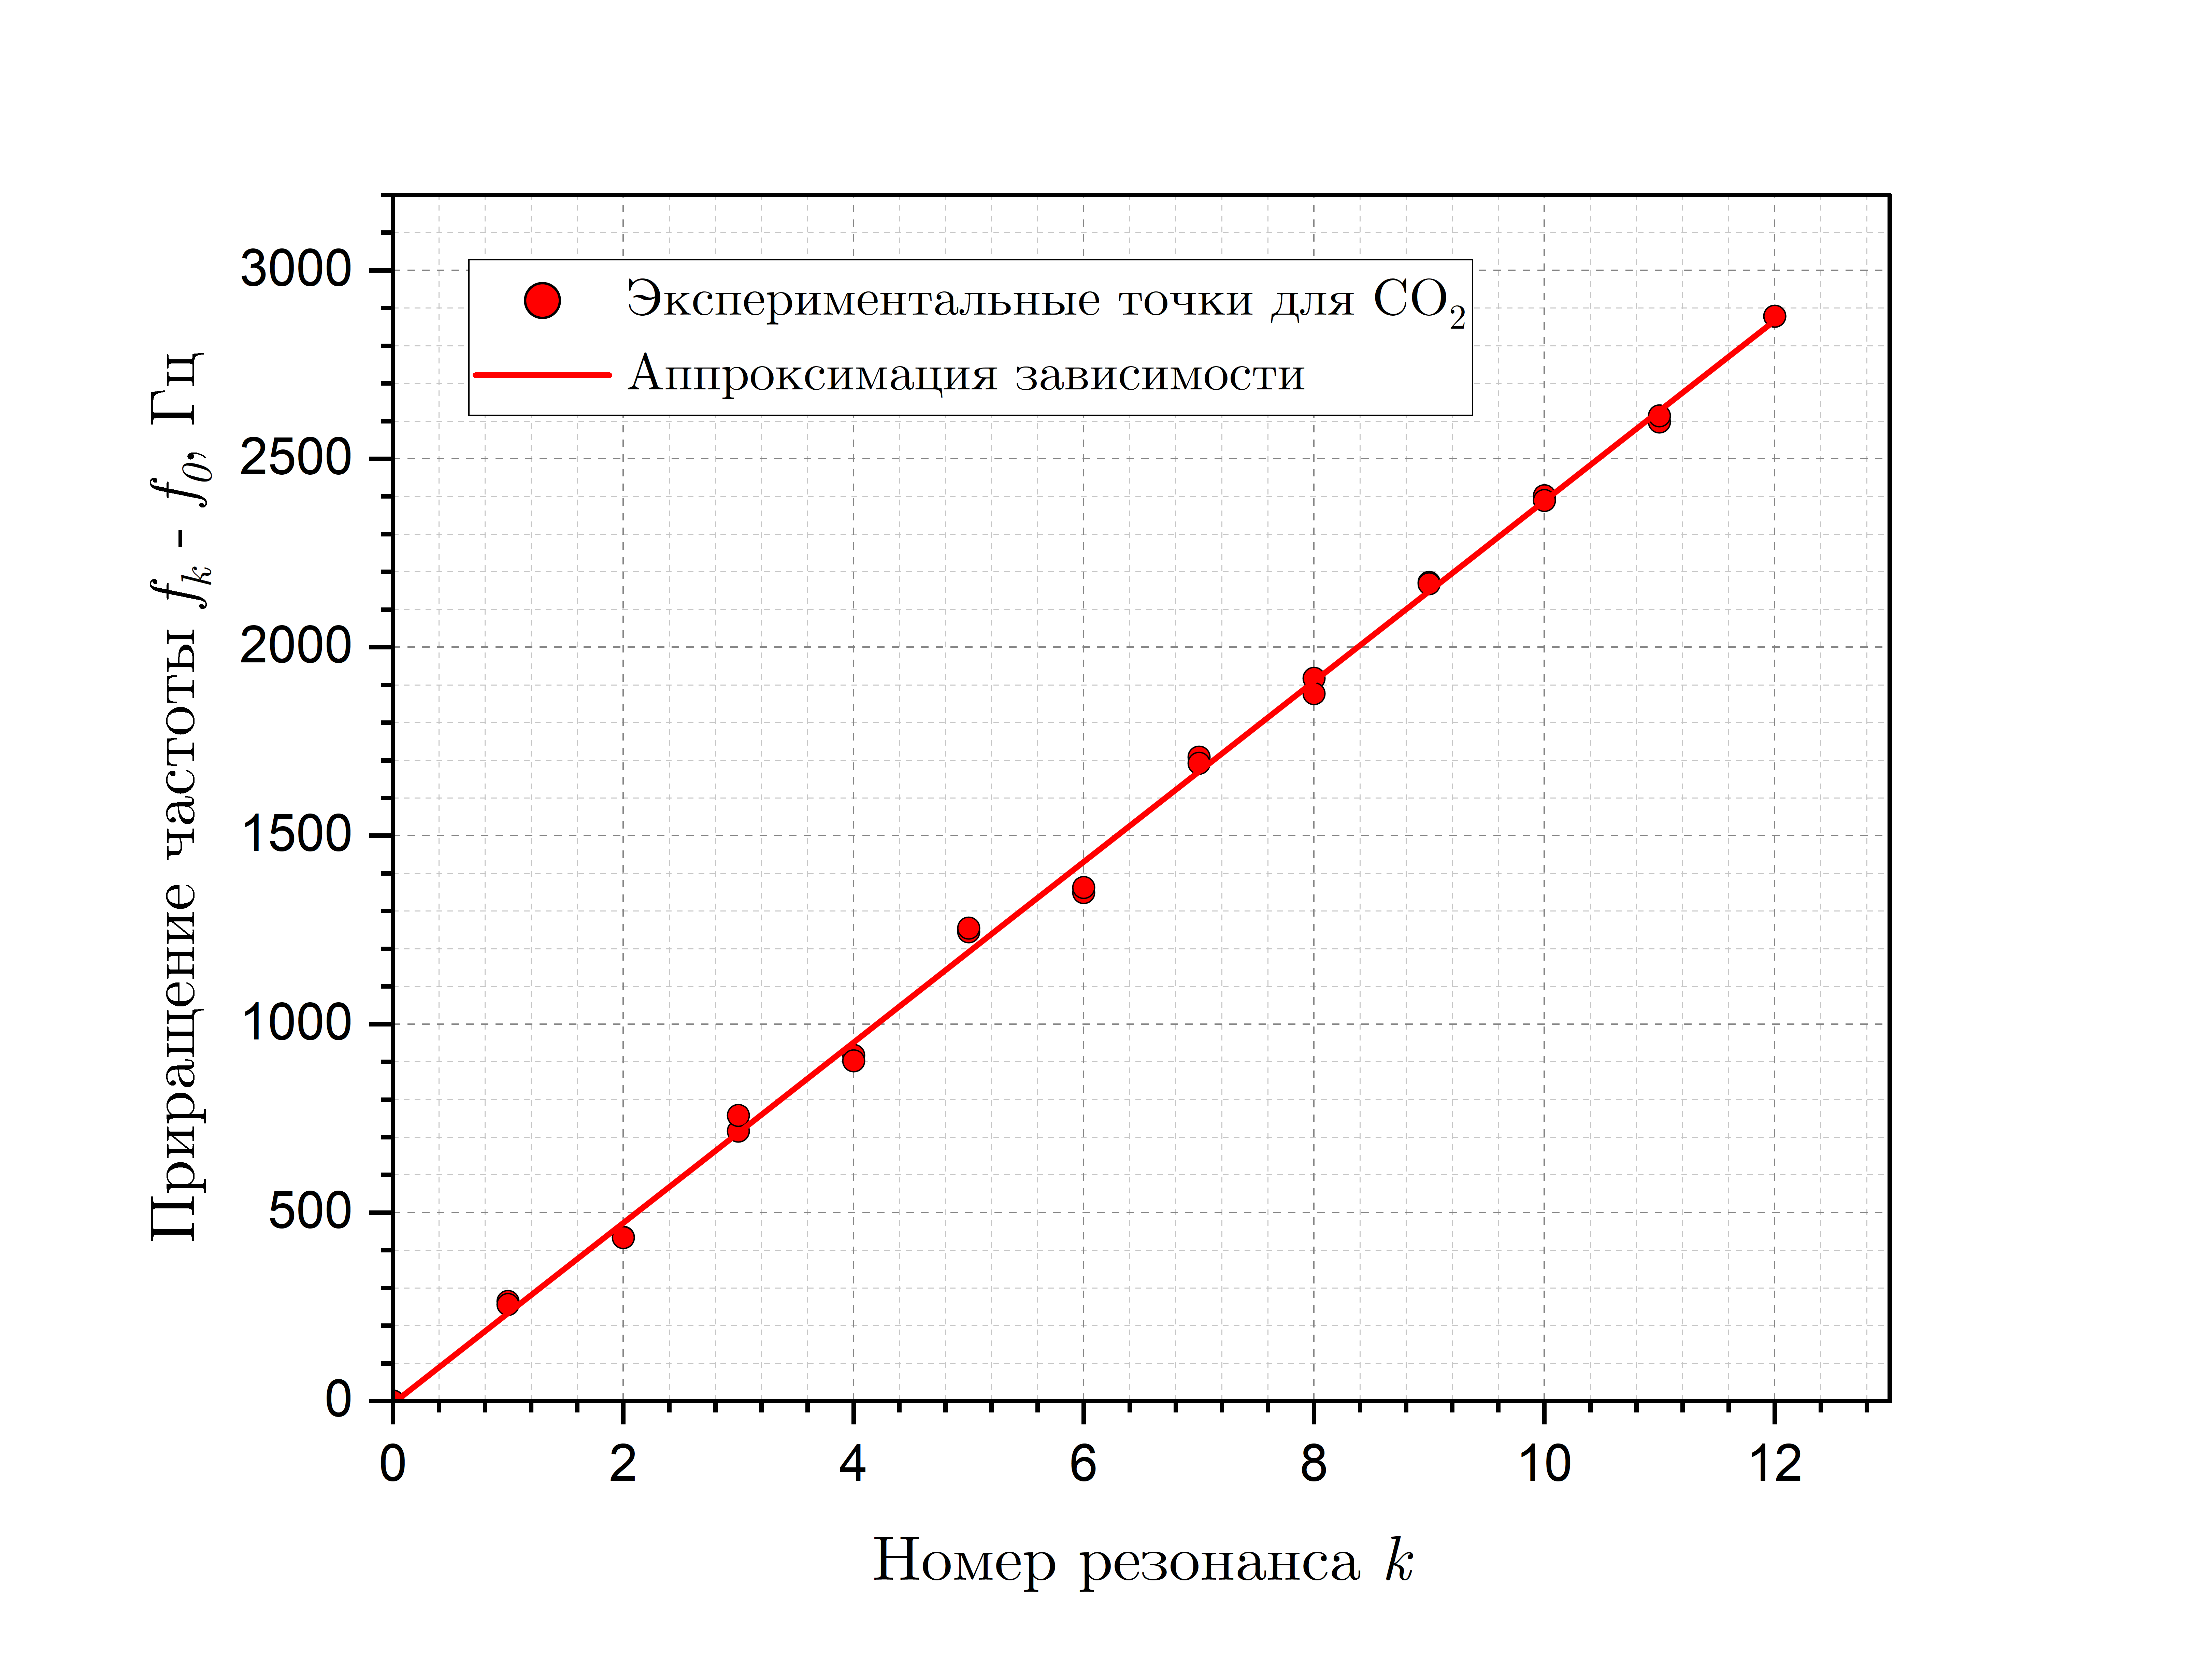
\includegraphics[scale = 0.5]{images/f(k)_CO2.png}
                \caption{График зависимости $\Delta f(k)$ для углекислого газа}
                \label{f(k)_CO2}
            \end{figure}

            \begin{figure}[H]
                \centering
                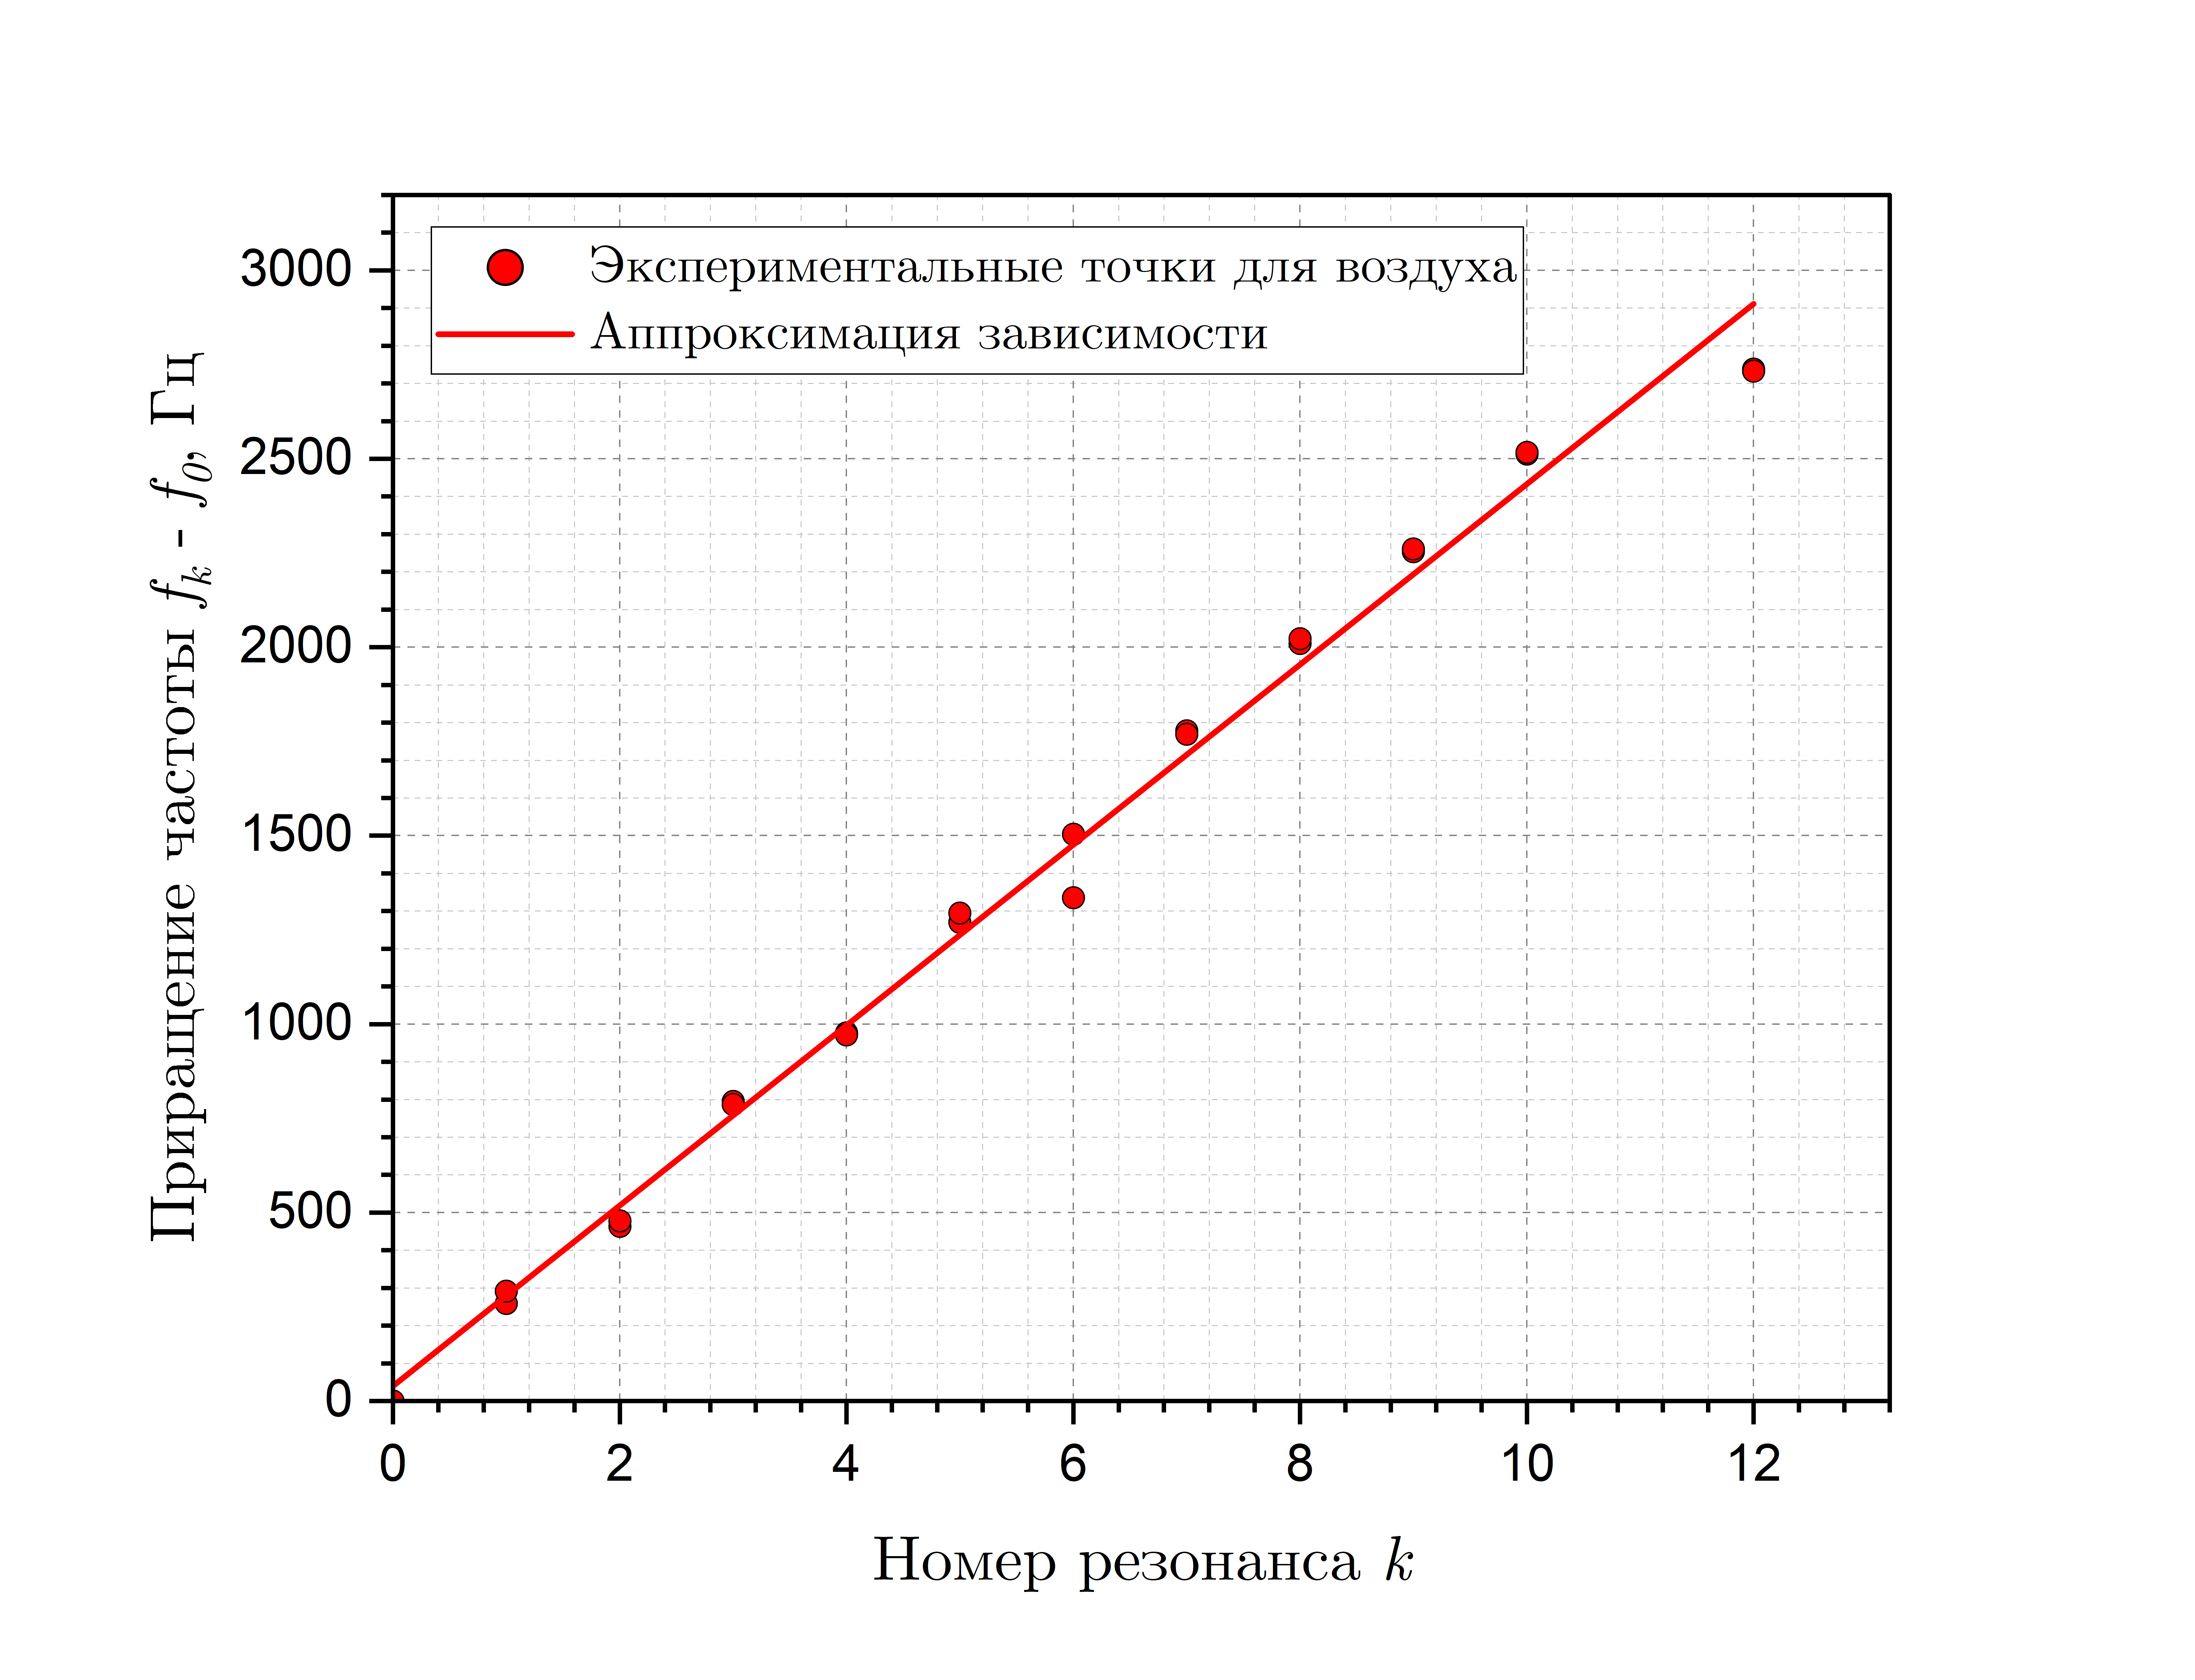
\includegraphics[scale = 0.5]{images/f(k)_oxy.png}
                \caption{График зависимости $\Delta f(k)$ для воздуха}
                \label{f(k)_oxy}
            \end{figure}

            \noindent Аппроксимируем полученные зависимости прямыми $y=ax$ используя метод наименьших квадратов. Коэффициент $a$ и погрешности его определения находим по приведенным в предыдущих пунктах формулам.\\

            \noindent Коэффициент наклона $\displaystyle a = \frac{c}{2L}$. Тогда вычислим скорость звука $c$ при фиксированной температуре и её погрешность. Кроме того, по формуле \eqref{gamma} вычислим $\gamma$ при фиксированной температуре и погрешность этого вычисления. 

            \noindent Получим: $a_{\text{возд}} = 239,3 \pm 4,4$ Гц и $a_{CO_2} = 239,4 \pm 1,97$ Гц. Следовательно,
            $$
            \boxed{c_{\text{возд}} = 335 \pm 7 \text{ м/с} \: (\varepsilon = 2 \%); \: c_{CO_2} = 335 \pm 4 \text{ м/с} \: (\varepsilon = 1,2 \%)}
            $$

            \noindent Отсюда,
            $$
            \boxed{\gamma_{\text{возд}} = 1,32 \pm 0,04 \text{ м/с} \: (\varepsilon = 2,8 \%); \: \gamma_{CO_2} = 2,00 \pm 0,07 \text{ м/с} \: (\varepsilon = 1,7 \%)}
            $$


    \section*{Заключение}
        \noindent В ходе работы показатель адиабаты для воздуха был измерен двумя разными способами. Сначала измерения проводились при фиксированной частоте звукового сигнала, а мы изменяли длину трубы. В ходе таких измерения было получено:

        \[ \boxed{\gamma_f = 1,37 \pm 0,03}\quad (\varepsilon=1,5\%) \]

        \noindent Сравним полученные данные с табличными. Согласно справочнику, показатель адиабаты для воздуха при нормальных условиях равен \underline{$\gamma = 1,4$}. Таким образом, можно утверждать, что результат измерения $\gamma$ на первой установке в пределах погрешности совпадает с табличными данными. Результаты измерения на второй установке незначительно отличаются от табличных. Это может быть связано с большой неточностью определения резонансных частот на второй установке. Чтобы этого избежать, необходимо использовать генератор частоты с возможностью более точной настройки для возможности чёткого отслеживания резонансов.

        \noindent Также в ходе работы был измерен показатель адиабаты для углекислого газа. Измерения проводились на первой установке. В итоге мы получили \[ \boxed{\gamma_{CO_2} = 1,88\pm 0,06}\quad (\varepsilon=3,3\%) \]

        \noindent Сравним эти данные с табличными. Согласно справочнику, показатель адиабаты для углекислого газа при нормальных условиях \underline{$ \gamma = 1,3 $}. Таким образом, полученные данные значительно отличаются от табличных. Это связано с тем, что при измерениях в трубе находился углекислый газ с примесями (в основном, азот и кислород), которые исказили результаты измерений (как оказалось, балон с углекислым газом был пуст).

\end{document}